% ============================================================
% Phase 4 — Non-symbolic Models
% ============================================================
 
\documentclass[11pt,a4paper]{article}
 
\usepackage[utf8]{inputenc}
\usepackage[T1]{fontenc}
\usepackage[a4paper,margin=2.5cm]{geometry}
\usepackage{booktabs}
\usepackage{graphicx}
\usepackage{float}
\usepackage[hidelinks]{hyperref}
\usepackage[style=apa,backend=biber]{biblatex}
 
\addbibresource{references.bib}
 
\begin{document}
 
\section{Non-symbolic Models}
 
After the Decision Tree, we trained four non-symbolic models: Random Forest, XGBoost, LightGBM, and MLP (Multi-Layer Perceptron, a small neural network). Our goal was to cover the main model families used for tabular data: bagging (Random Forest), boosting (XGBoost and LightGBM, with different tree growth strategies), and neural networks (MLP). The first three models are all built on Decision Trees, just combined in different ways. MLP is something completely different. We added it because we wanted at least one model from outside the tree family for comparison.
 
\subsection{Setup}
 
To keep things consistent with the Decision Tree, we used the same 80/20 split with \texttt{random\_state = 42}. In this way, the train and test sets contain exactly the same buildings as in the Decision Tree notebook, so the RMSE values can be directly compared without worrying that differences are caused by different data splits. The missing values were filled in with the median. An extra step we needed for MLP was \texttt{StandardScaler}, since neural networks do not really work without scaled inputs. The tree-based models do not care about this, so we skipped scaling for them.

We evaluated everything with 10-fold cross-validation on the training set. RMSE is our main metric, MAE is a secondary one. For tuning, we went with \texttt{RandomizedSearchCV}. A full grid search would have taken forever, given how many parameters each model has, so we let it pick 30 random combinations for the tree models. For MLP, we only did 20 since each fit takes longer.
 
\subsection{Results}
 
Our cross-validation results are in Table~\ref{tab:results}.
 
\begin{table}[H]
\centering
\caption{Cross-Validation Results}
\label{tab:results}
\begin{tabular}{lcc}
\toprule
Model                     & CV RMSE          & CV MAE \\
\midrule
Decision Tree (tuned)     & 5.980            & 4.061 \\
\addlinespace
Random Forest (default)   & 5.693            & 3.758 \\
Random Forest (tuned)     & 5.416            & 3.616 \\
XGBoost (default)         & 5.564            & 3.822 \\
XGBoost (tuned)           & \textbf{5.354}   & \textbf{3.600} \\
LightGBM (default)        & 5.770            & 4.013 \\
LightGBM (tuned)          & 5.361            & 3.624 \\
MLP (default)             & 5.871            & 4.052 \\
MLP (tuned)               & 5.762            & 3.946 \\
\bottomrule
\end{tabular}
\end{table}
 
Every non-symbolic model beat the tuned Decision Tree. The best one was XGBoost with an RMSE of 5.354 and MAE of 3.600. Since EPC scores range from 1 to 147, an average error of about 5.4 means our predictions are usually within a single rating band of the actual value. LightGBM came in basically tied with XGBoost (only 0.007 behind on RMSE), which we expected since they are both gradient boosting algorithms. Random Forest was next, about 0.06 RMSE behind LightGBM, and MLP was the worst of the four, with around 0.4 higher error.

Tuning gave each model some improvement, but the gains were modest, usually around 0.2 to 0.4 RMSE points. This suggests that the default settings of these libraries are already well chosen for tabular data like ours.
 
Table~\ref{tab:params} shows the best parameters we ended up with for each model.
 
\begin{table}[H]
\centering
\caption{Best Parameters from RandomizedSearchCV}
\label{tab:params}
\small
\begin{tabular}{ll}
\toprule
Model         & Best parameters \\
\midrule
Random Forest & \texttt{n\_estimators=300}, \texttt{max\_depth=20}, \\
              & \texttt{max\_features=0.5} \\
\addlinespace
XGBoost       & \texttt{n\_estimators=500}, \texttt{max\_depth=10}, \\
              & \texttt{learning\_rate=0.1}, \texttt{subsample=1.0} \\
\addlinespace
LightGBM      & \texttt{n\_estimators=1000}, \texttt{num\_leaves=127}, \\
              & \texttt{learning\_rate=0.05} \\
\addlinespace
MLP           & \texttt{hidden\_layer\_sizes=(150,100,50)}, \\
              & \texttt{activation=tanh}, \texttt{alpha=0.01} \\
\bottomrule
\end{tabular}
\end{table}
 
\subsection{Feature Importance}
 
Figure~\ref{fig:fi} shows the top 15 features for each of the tree-based models. We left MLP out of this one because neural networks do not give feature importance the same way trees do.
 
\begin{figure}[H]
\centering
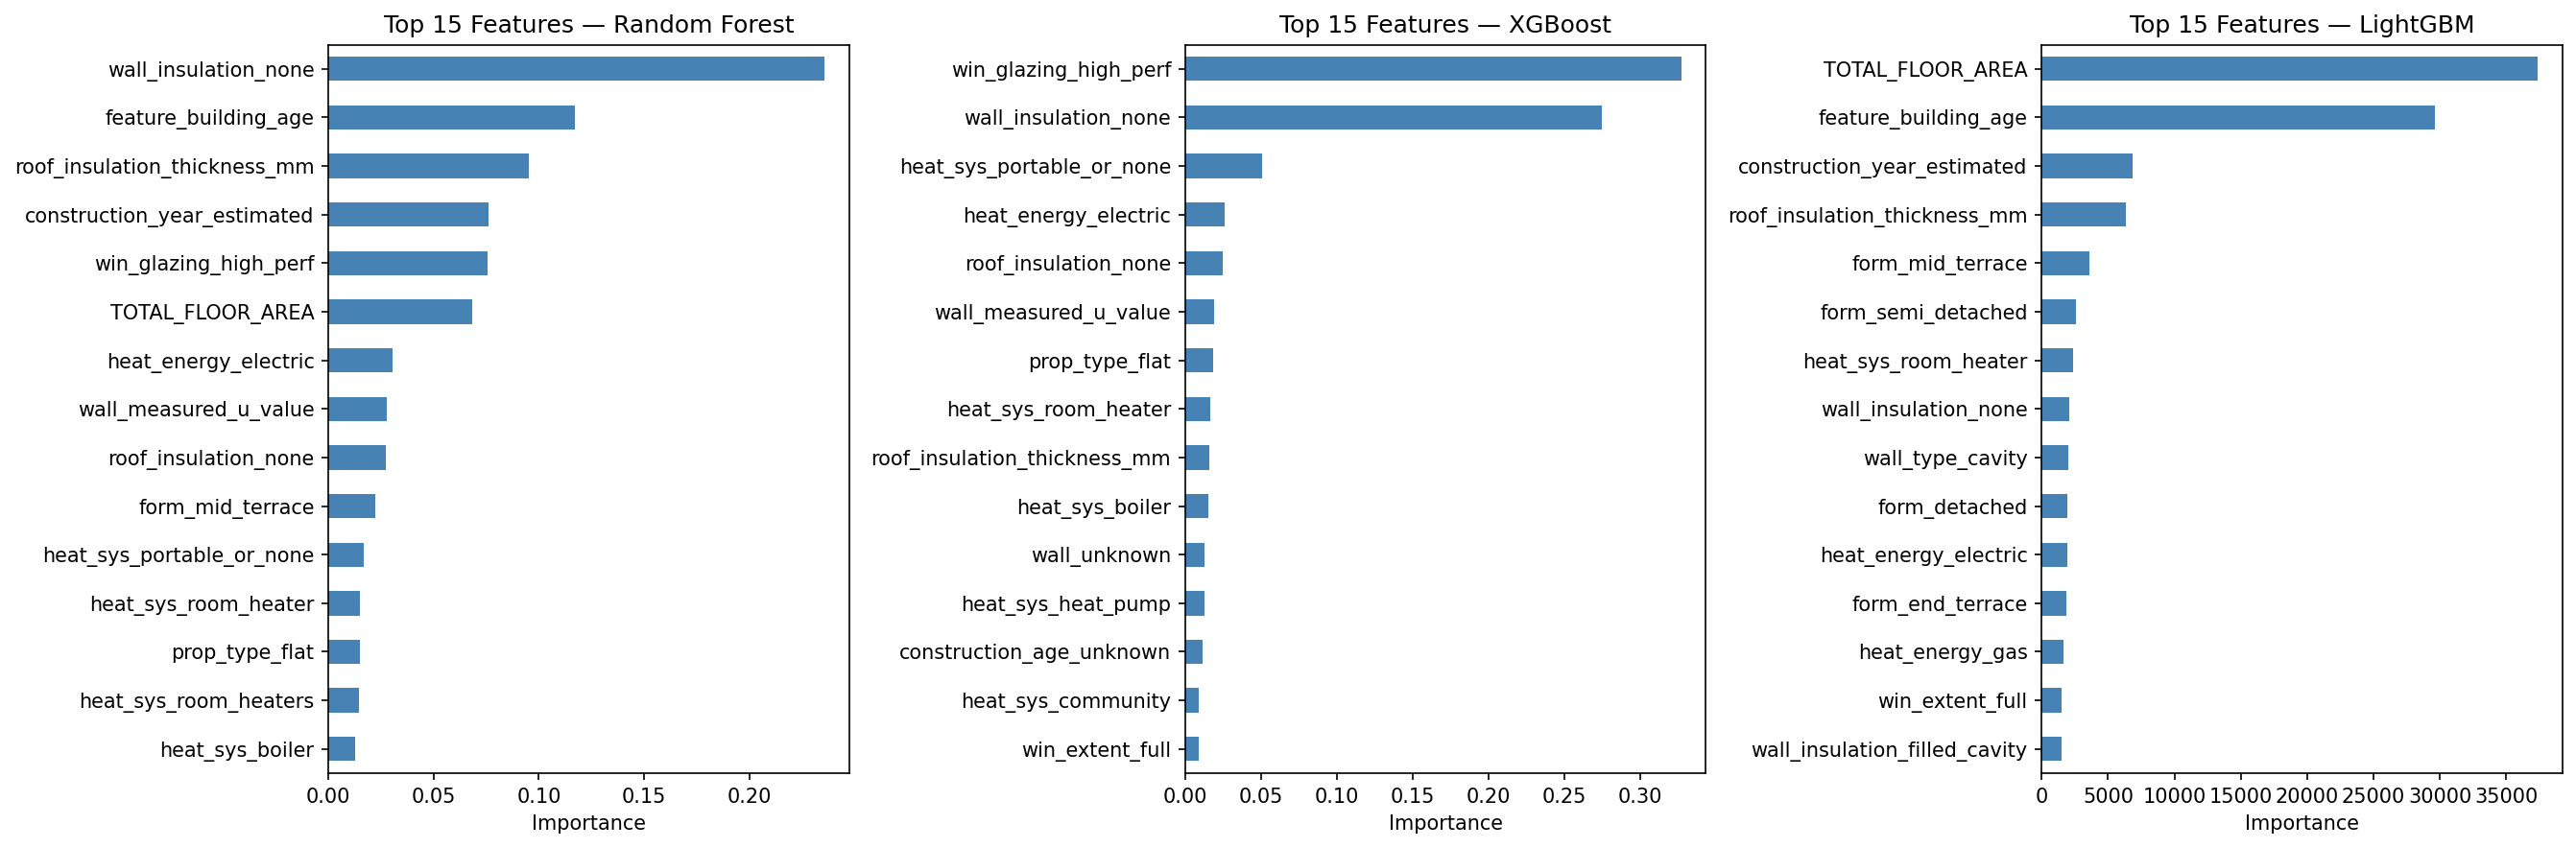
\includegraphics[width=\textwidth]{nonsymbolic_feature_importance.png}
\caption{Top 15 features for Random Forest, XGBoost, and LightGBM.}
\label{fig:fi}
\end{figure}
 
Looking at the three plots, all of the models highlight the same top features: wall insulation, building age, roof insulation thickness, glazing type, and floor area. These are also the same features the Decision Tree identified as important. That gave us some confidence that the models
are learning real patterns in the data rather than just memorizing noise.
 
\subsection{Discussion}
 
Going from the Decision Tree (5.980) to XGBoost (5.354) is about a 10.5\% drop in error, which is a noticeable improvement. It makes sense too, since combining a lot of trees should give us more flexibility than relying on just one.
 
XGBoost and LightGBM finished almost tied, and that is mostly because they are built on the same idea (gradient boosting). The small gap is probably due to how they grow trees internally and their default regularization. Random Forest was a bit further behind, but in fairness, it is also a different approach (bagging instead of boosting), and it needed less tuning to get to a decent result.
 
The MLP was the most disappointing for us. Even after tuning the layer sizes, activation, learning rate, and regularization, it could not catch up to the gradient boosting models. We did some reading on this and found that this is actually a known thing. On tabular datasets like ours, tree-based models tend to outperform neural networks pretty consistently \parencite{grinsztajn2022tree}. Neural networks usually show their strength on images, text, or audio, not on structured data like building characteristics.
 
One thing worth mentioning is interpretability. The decision tree was easy to explain because you can read the rules directly from it. The non-symbolic models do not work like that. They are more of a black box. The feature importance plots help a bit, but in Evaluation we plan to use SHAP on XGBoost so we can explain individual predictions instead of just looking at overall feature rankings.
 
\printbibliography
 
\end{document}
